\documentclass[
]{ceurart}

\sloppy
\usepackage{svg}
\usepackage{listings}
\lstset{breaklines=true}
\usepackage{todonotes}
\usepackage[justification=centering]{caption}


\begin{document}

\copyrightyear{2023}
\copyrightclause{Copyright for this paper by its authors.
  Use permitted under Creative Commons License Attribution 4.0
  International (CC BY 4.0).}

\conference{Second International Workshop on Linked Data-driven Resilience Research (D2R2'23) co-located with ESWC 2023, May 28th, 2023, Hersonissos, Greece}

\title{Dynamic Representations of Global Crises: Creation And Analysis of a Temporal Knowledge Graph For Conflicts, Trade and Value Networks}

\author[1,2]{Julia Gastinger}[
email=julia.gastinger@neclab.eu,
]
\cormark[1]
\address[1]{NEC Laboratories Europe GmbH, Kurfuersten-Anlage 36, 69115 Heidelberg, Germany}
\address[2]{University of Mannheim, Data and Web Science Group, B 6, 26, 68159 Mannheim, Germany}

\author[3]{Nils Steinert}[
email=nils.steinert@implisense.com,
]
\address[3]{Implisense GmbH, Spiekermannstraße 31a, 13189 Berlin, Germany}

\author[4]{Sabine Gründer-Fahrer}[
email=gruender-fahrer@infai.org,
]
\author[4]{Michael Martin}[email=martin@infai.org]
\address[4]{Institute for Applied Informatics (InfAI), Goerdelerring 9, 04109 Leipzig, Germany}

\cortext[1]{Corresponding author.}

\begin{abstract}
This paper presents a novel approach to understanding global crises and trade patterns through the creation and analysis of a temporal Knowledge Graph (tKG). Combining data from the Armed Conflict Location \& Event Data Project (ACLED) and Global Trade Alerts (GTA), the tKG provides a comprehensive view of the intersection between worldwide crises and global trade over time. The paper details the process of creating the tKG, including the aggregation and merging of information from multiple sources. 
Additionally, the paper offers insights into the analysis of the tKG and its potential applicability to data-driven Resilience Research. As an initial application, the tKG can be used to predict global trade events, such as trade sanctions across various categories and countries, based on global conflict events, to identify potential trade disruptions and anticipate the economic impact of global conflicts.
\end{abstract}

\begin{keywords}
  Temporal Knowledge Graphs \sep
  Knowledge Graphs \sep
  Resilience Research \sep
  Crisis Research
\end{keywords}

\maketitle

\section{Introduction}\label{sec:intro}
\input{chapters/01_introduction.tex}

\section{Related Work}\label{sec:rel_work}
\subsection{Knowledge Graphs and Vocabularies for Resilience Research}
The use of Knowledge Graphs in resilience and crisis research has gained increasing attention in recent years \cite{Kim2022}. KG offer a flexible and comprehensive approach to modeling and analysing complex systems \cite{TILLY2021115765}, making them suitable for a wide range of domains, including macro-economical analysis \cite{Yang2020}, which is a main focus of the CoyPu research project.

Creating a KG requires a structured and standardized way to represent data in a machine-readable format. Ontologies offer a means to provide a shared vocabulary of terms and concepts that enable data to be integrated and analysed in a consistent and interoperable way. Although there exist established vocabularies \cite{Crofts2011} to model events, including their relevant actors, occurrence, locality, and other significant properties, the reuse of such vocabularies presents several challenges. These challenges arise from the complex, highly domain-specific nature of these vocabularies, divergent levels of granularity, lack of easy extensibility, and the difficulty of creating interoperable mappings between different ontologies. As a result, in the CoyPu project a custom ontology - the CoyPu COY ontology \cite{coy_2023} - was developed to model the KG.

\subsection{Temporal Knowledge Graph Datasets}  
\citet{Zhang2021} provide a comprehensive overview of existing temporal RDF models. We follow the work of \citet{Trivedi2017}, \citet{Li2021regcn}, \citet{Han2021xerte}, and others, who represent tKG as sequences of timestamped KG. A timestamped KG, or KG snapshot, denoted as $G_t = \{V,R, \mathcal{E}_t\}$, captures the state of the tKG at a specific timestep $t$, where $V$ is the set of entities, $R$ is the set of relations, and $\mathcal{E}_t$ is the set of quadruples \cite{Li2021regcn}. A quadruple consists of four elements, such as \textit{(Event A, hasActor, French Police Forces, 2021-07-01)}. 

In the domain of tKG analysis, six datasets have been published and utilized, including different versions of the Integrated Crisis and Early Warning System (ICEWS) \cite{Boschee2015}: ICEWS05-15 \cite{GarciaDuran2018ICEWS14}, ICEWS14 \cite{GarciaDuran2018ICEWS14}, and ICEWS18 \cite{Jin2019oldrenet} (the numbers describe the respective years); GDELT \cite{Leetaru2013GDELT}; YAGO \cite{Mahdisoltani2015YAGO}; and WIKI \cite{Leblay2018WIKI} (preprocessed by \citet{Jin2019oldrenet}). Notably, the three versions of ICEWS cover the crisis topic, demonstrating the applicability of tKG to crisis research. However, to the best of our knowledge, no tKG currently exists that describes trade relations and sanctions over time. Additionally, none of the existing tKG merge data from multiple sources to provide a comprehensive view or analyse the interconnection of different event types. Finally, to our knowledge, no other study has analysed the evolution of graph properties over time for tKG.


\section{Resources}\label{sec:resources}
\subsection{GTA}
The Global Trade Alerts (GTA) dataset~\cite{gta_paper} is a comprehensive database that tracks trade-related policy measures implemented by nation-states around the world since 2008. The dataset contains a wide range of measures, including tariff and non-tariff barriers, export taxes and subsidies, import measures, and other trade-related policies.
It is updated in real-time and is provided as open data\footnote{\url{https://www.globaltradealert.org/}}. 

One of the key strengths of the GTA dataset is its focus on the affected jurisdictions, providing details on both the implementing and the affected jurisdiction for each measure. Additionally, it covers measures that impact the flow of goods and services across borders, such as taxation and exim quotas. Moreover, GTA provides information on the broader context of each measure, including the sectors and industries that are most affected by their implementation, as well regulatory political and economic factors that may be driving changes in trade policy. Overall, these aspects allow for analysing the impact of trade regulations on specific countries or regions, and to identify patterns and trends in trade policy over time on the global economy.

\subsection{ACLED}
The Armed Conflict Location \& Event Data Project (ACLED)~\cite{acled_paper} is a non-profit organization that collects and analyses data on political violence and protest events across the world.

ACLED uses a combination of media monitoring, crowd-sourcing, and other open-source data collection methods to track and record information about incidents of political violence, including battles, bombings, riots, and protests. The organization's database covers more than 200 countries and provides information on the actors involved in each conflict, as well as the location, date, type, and intensity of the violence. The dataset is updated weekly and can be accessed via an API or downloaded as a data dump\footnote{\url{https://acleddata.com/data-export-tool/}}.

\subsection{Relationships between GTA and ACLED}
There are several possible relationships and dependencies between the ACLED dataset and the GTA dataset, e.g.:
\begin{description}
    \item[ACLED events can lead to trade sanctions] If a country experiences political violence or conflict, other countries may respond by imposing trade sanctions or embargoes. For example, if a country is involved in a civil war, other countries may decide to stop trading with it. % until the conflict is resolved. 
    In this case, ACLED informs on the political violence that led to the sanctions, while GTA tracks the implemented trade policies.
    \item[Trade policies can exacerbate conflicts] Trade policies can sometimes exacerbate political conflicts or tensions between countries. E.g., the trade restrictions that one country imposes on another could lead to economic hardship and political instability, which could in turn lead to conflicts. In this case, GTA informs on the trade policies that contributed to the conflict, while ACLED tracks the specific instances of violence or unrest.
    \item[ACLED events can disrupt trade flows] Political violence or unrest can disrupt trade flows between countries. For example, an attack on a major transportation hub could lead to delays or disruptions in trade. In this case, ACLED informs on the incidents of violence that disrupted trade flows, while GTA tracks the affected trade policies or agreements.
\end{description}

Overall, using the ACLED and GTA datasets together provides a comprehensive picture of the relationship between political conflict and international trade.
By analysing these datasets in tandem, policymakers and researchers can better understand the ways in which political violence and trade policies are interconnected, and develop more effective strategies for promoting peace and economic growth.


\section{Method and Implementation}\label{sec:method}
The creation of the present temporal Knowledge Graph, which comprises a subset of the larger CoyPu KG, involves several steps to integrate the data into a structured and standardized framework. 

First, the source data is retrieved manually from the corresponding web services in a machine-readable format. Next, the data is converted into RDF format using an ontology schema that defines the relevant concepts, properties, and relationships. This enables the representation of the source data as a set of triples and allows for its integration with other RDF data sources. 
Both the ALCED and GTA datasets are mapped to RDF based on custom ontology declarations. These declarations contain the specific semantic specifications of transforming the source data into triples and form an extension of the central CoyPu COY ontology \cite{coy_2023}. 
We provide both the ontology OWL files, as well as the RML mapping rules used for the graph creation process in our repository for reproducibility.

\begin{description}
\item[Simplification] We aim to simplify the ACLED and GTA datasets to extract relevant information for our use case, while minimizing noise from irrelevant information. Thus, for GTA, we exclude triples that contain labels, intervention and state acts IDs, and event types, as these triples do not provide any additional information. For ACLED, we exclude triples with comments and labels, and only consider the country location of each event.

\item[Aggregation]
GTA uses the hierarchical industry classification schemes \textit{CPC 2.1} and \textit{HS 2012} to denote the affected sectors and products of an intervention. These schemes may include a very large number of categories, making the analysis more challenging. To address this issue, we use broader sector and product categories, based on higher-level groupings within the respective classification scheme. E.g., instead of considering each individual product category, we group products into broader categories based on their use or production process, such as "primary agricultural products". This is useful for modeling the impact of political violence or other events on trade flows, as it helps to identify the most affected sectors or products. 
As this data reduction is helpful in our use case but could be harmful in others, it is a configurable step during dataset generation.  
\item[Merging GTA and ACLED] The GTA and ACLED events can be linked via their annotated country information. In GTA, country data is available for the implementing and the affected jurisdiction of each intervention or state act. Meanwhile, in ACLED, country information is available from the locations of involved actors and of the ACLED events themselves. We illustrate such a connection in Figure~\ref{fig:link}, depicting two ACLED events and a GTA intervention in Ukraine and Russia in 2021. It is important to note that this link does not necessitate causality, but rather serves as a foundation for further analysis.

\begin{figure}
    \centering
    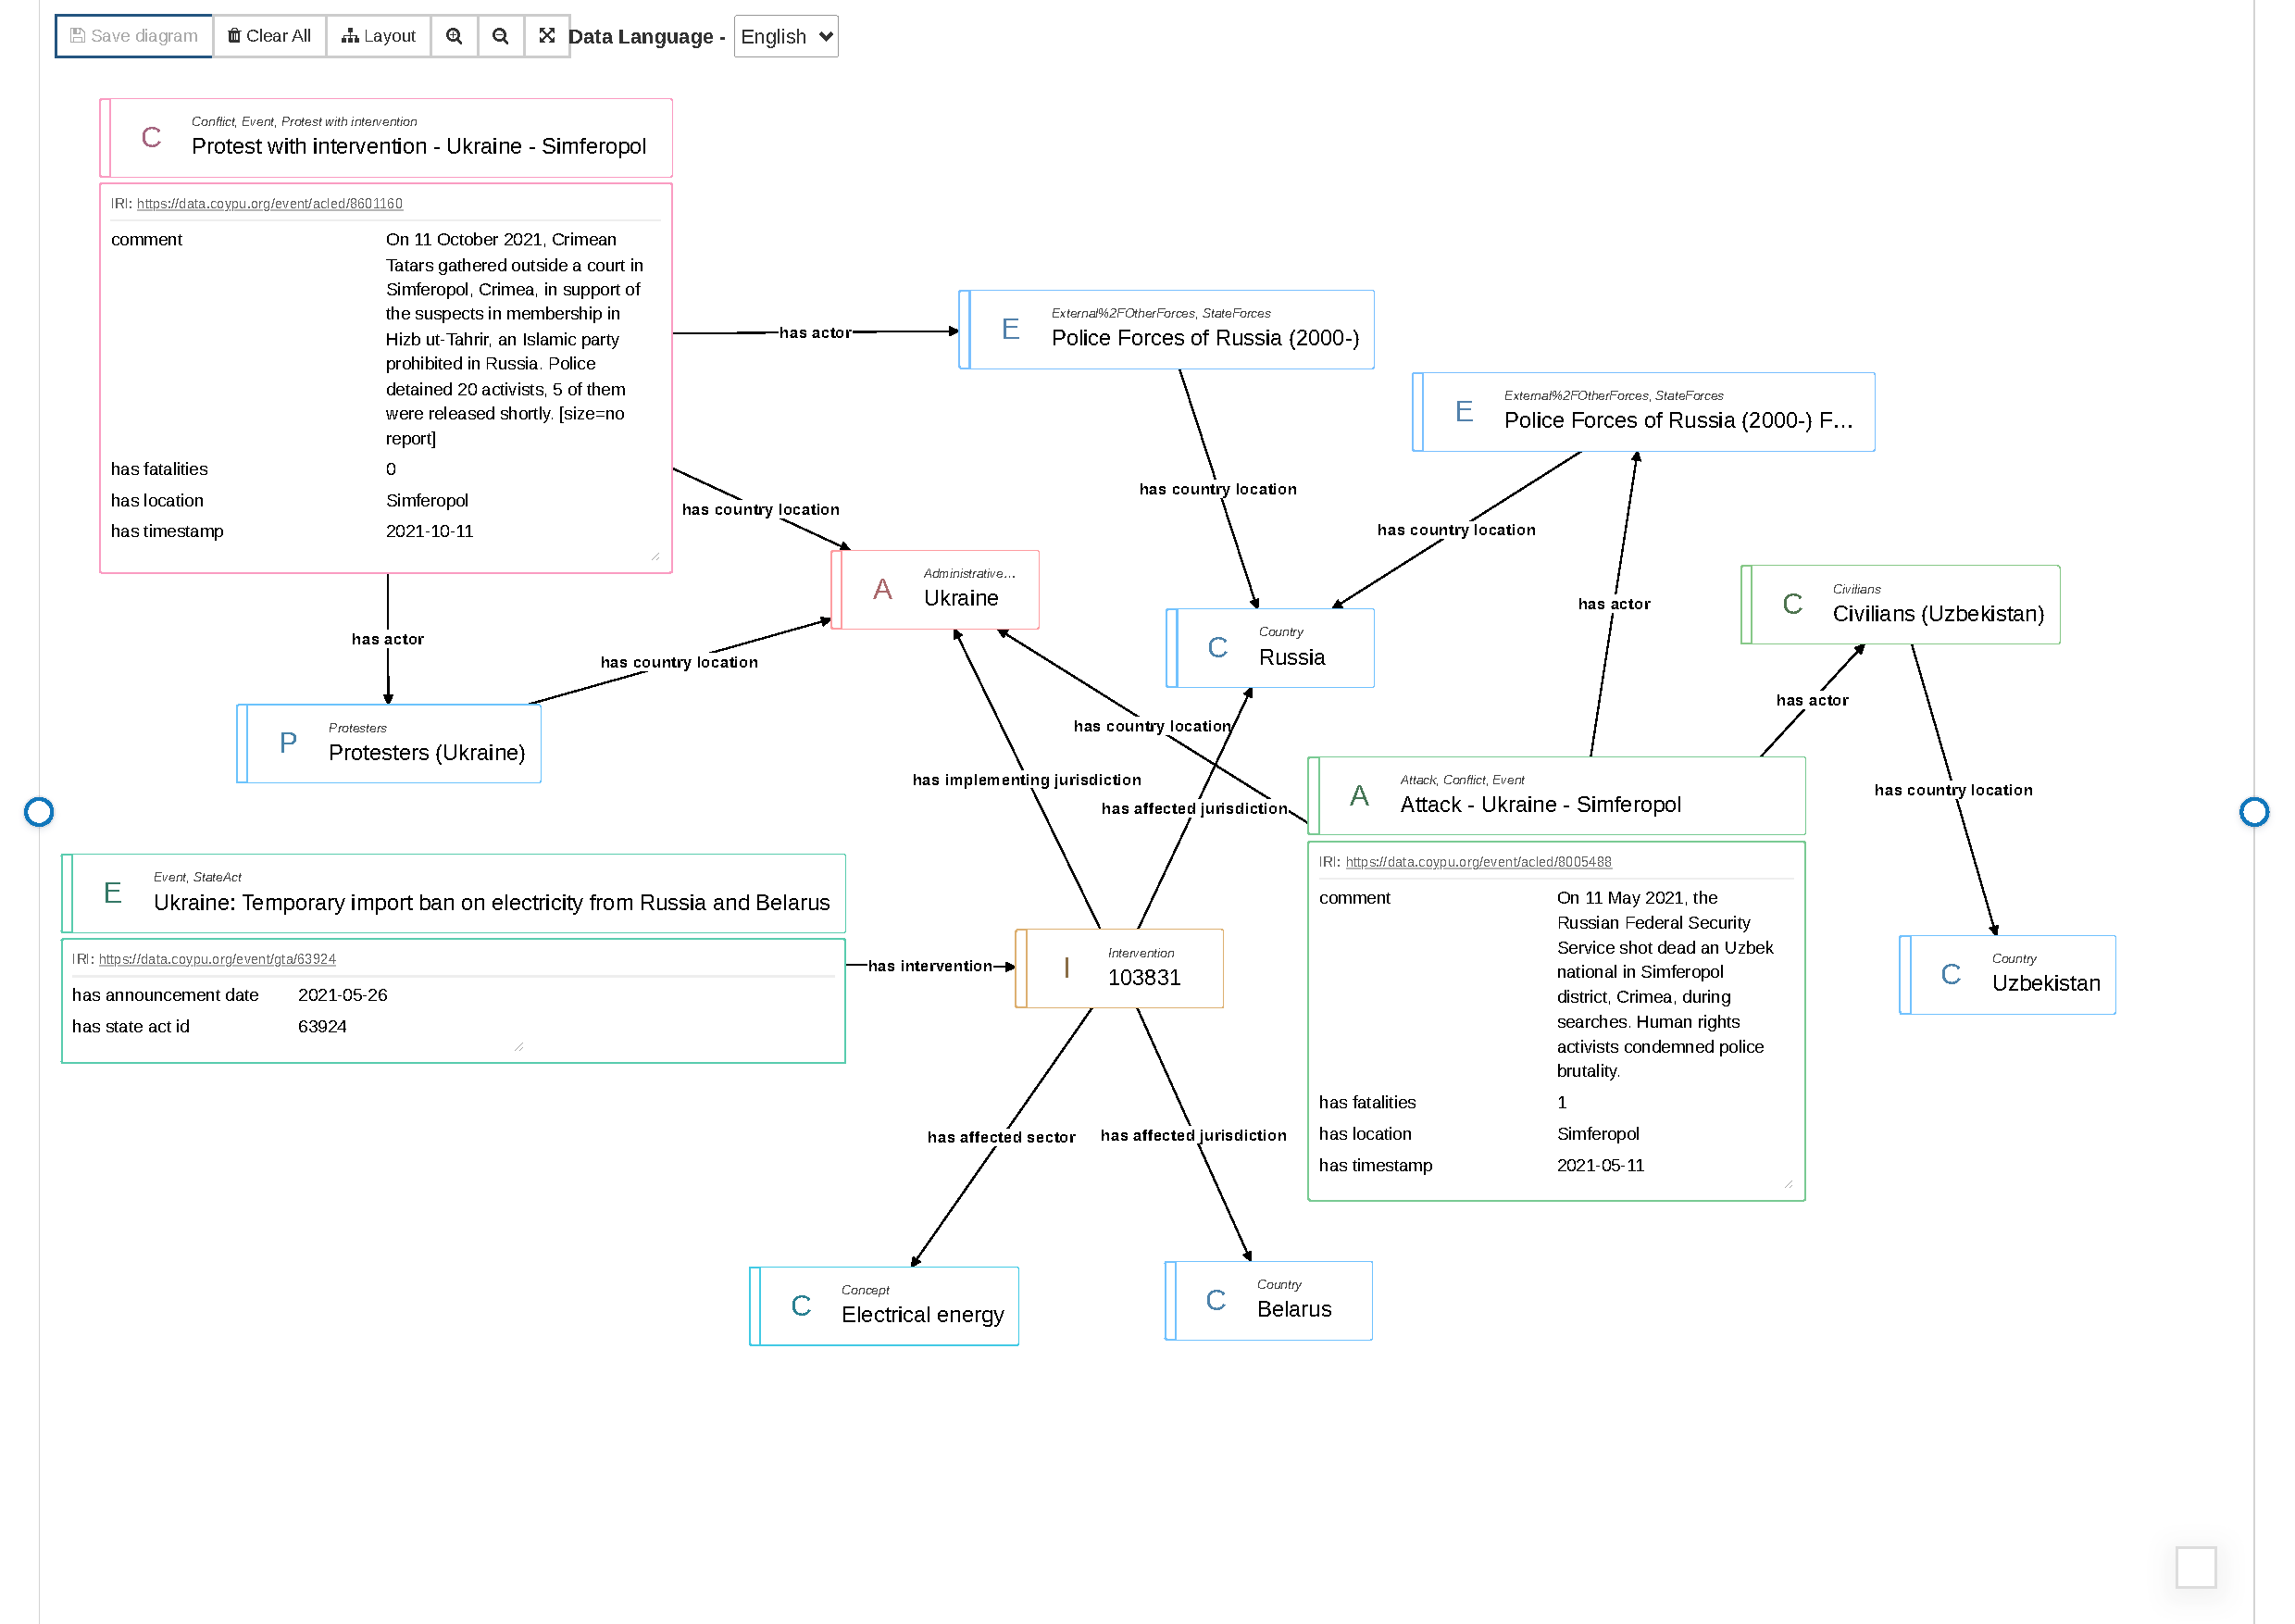
\includegraphics[clip, trim=1.1cm 5.0cm 1.2cm 1.8cm, width=0.7\textwidth]{figs/acled_gta.pdf}
    \caption{Link between two ACLED events and a GTA event via locations in 2021. The ACLED events (\textit{Attack - Ukraine - Simferopol}, green, and \textit{Protest with intervention - Ukraine - Simferopol}, pink) and the GTA intervention (\textit{intervention 103831}, yellow) link via Russia and Ukraine. }
    \label{fig:link}
\end{figure}

\item[Temporal Information] 
From the given graph in RDF format, we create a tKG with daily granularity, containing quadruples for each day in the year 2021. We have opted to utilize quadruples as our chosen representation, as they are widely employed in the field of tKG forecasting research, see e.g., \cite{Jin2019oldrenet}, \cite{Li2021regcn}, \cite{Han2021xerte}.
ACLED provides daily timestamps for each event. We create the quadruples by adding this timestamp data to all triples that are connected to this event. 
GTA provides an announcement date of each state act, as well as the implementation date, and - if existing - the removal date for each connected intervention. 
Since our use case (see Section~\ref{sec:UseCase}) aims to predict upcoming global trade events, we focus on the earliest available date for each GTA event, i.e. the announcement date. Therefore, we add the announcement date timestamp to all triples belonging to a state act or intervention. 
The output of this step is a tKG with quadruples in TXT format for further analysis. 
\end{description}


\section{Analysis and Results}\label{sec:experiments}
Following the steps outlined in Section~\ref{sec:method} results in a tKG comprising 1,513,398 quadruples across 365 timesteps, with 290,457 distinct nodes and 13 distinct relations. In this tKG, 1,424,956 quadruples originate from the ACLED dataset, 88,442 quadruples originate from the GTA dataset, containing information on in total 3,677 GTA interventions. In the following, we describe this tKG and provide insights from the conducted analysis.

\subsection{Temporal Knowledge Graph Analysis} 
We analyse the resulting tKG by computing and observing its graph properties over time. Figure~\ref{fig:graph_params_timeseries} illustrates these properties of the KG snapshots per timestep, including the number of triples (a), the number of nodes (b), the density (c), the mean node degree (d), and the maximum node degree (e). 
\begin{figure*}[!t]
\begin{minipage}{\textwidth}
	\centering
	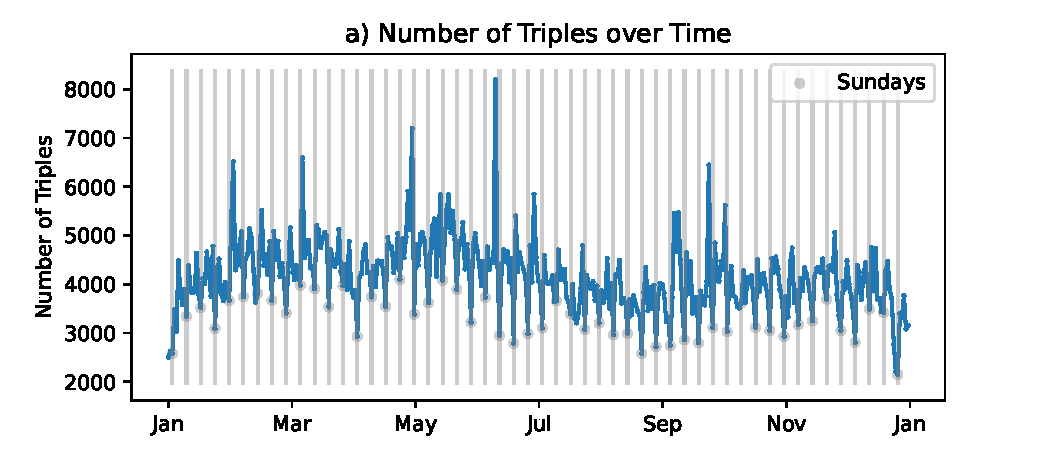
\includegraphics[width=0.43\textwidth]{figs/acled_subset_gta_aggregatedNumber of Triples.pdf}\\
\end{minipage}
\begin{minipage}{0.43\textwidth}
	\centering
	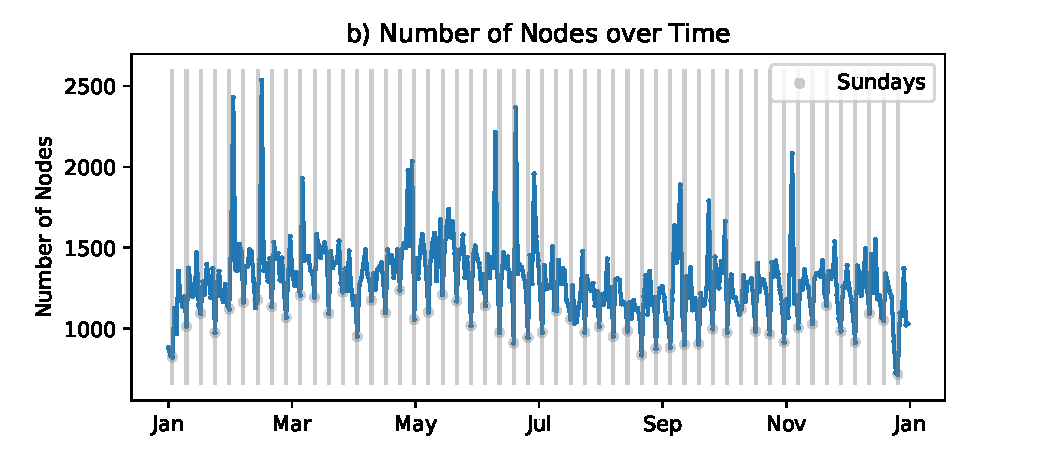
\includegraphics[width=\textwidth]{figs/acled_subset_gta_aggregatedNumber of Nodes.pdf}\\
\end{minipage}
\hfill
\begin{minipage}{0.43\textwidth}
	\centering
	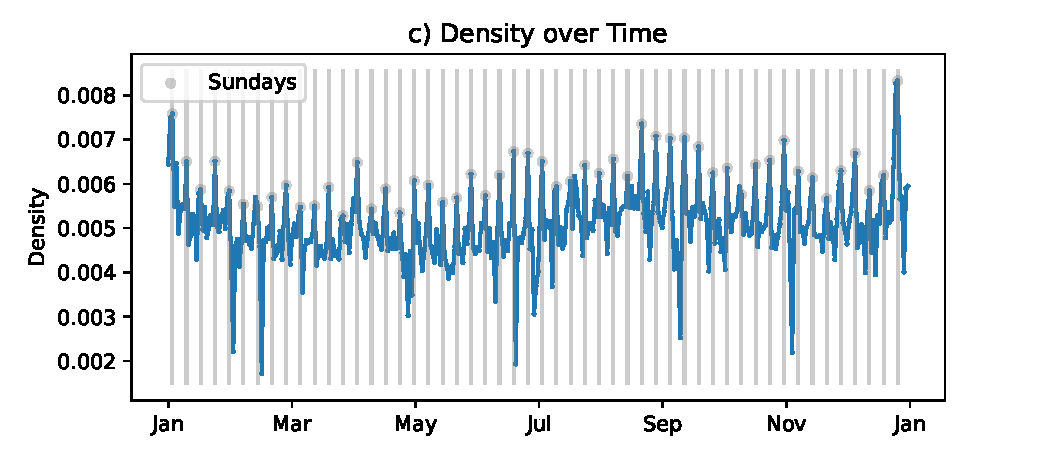
\includegraphics[width=\textwidth]{figs/acled_subset_gta_aggregatedDensity.pdf}\\
\end{minipage}
\begin{minipage}{0.43\textwidth}
	\centering
	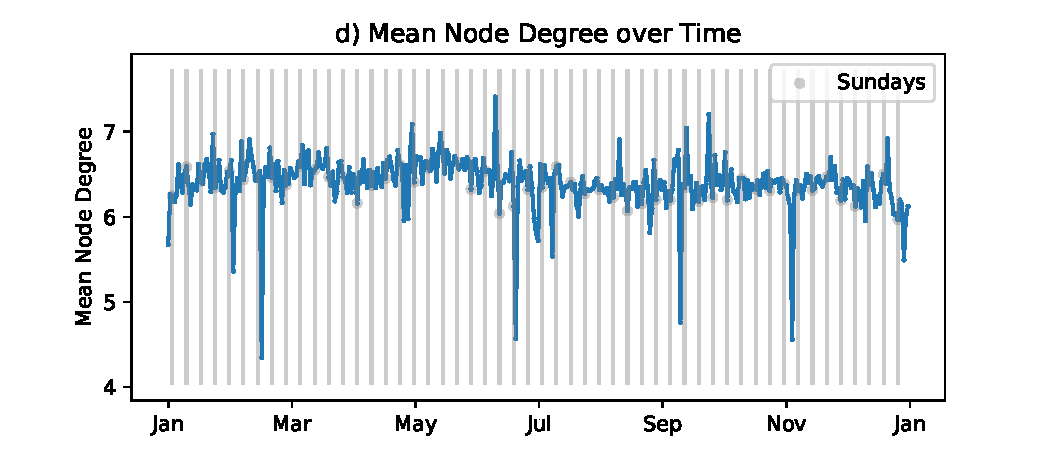
\includegraphics[width=\textwidth]{figs/acled_subset_gta_aggregatedMean Node Degree.pdf}\\
\end{minipage}
\hfill
\begin{minipage}{0.43\textwidth}
	\centering
	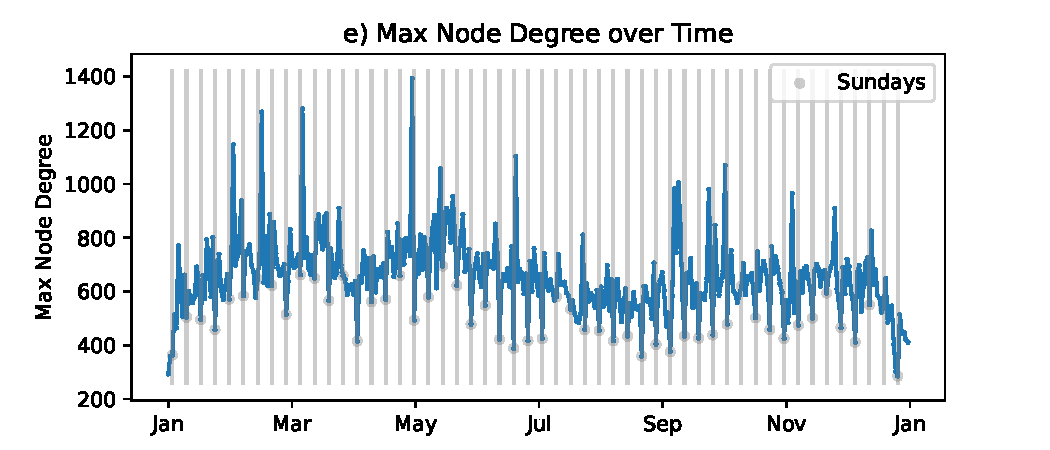
\includegraphics[width=\textwidth]{figs/acled_subset_gta_aggregatedMax Node Degree.pdf}\\
\end{minipage}
\caption{Graph properties over time, one entry per graph snapshot. All Figures show the year 2021. 
Grey lines and dots mark Sundays. (a) number of triples, (b) number of nodes, (c) density, (d) mean node degree, (e) max node degree.}  
\label{fig:graph_params_timeseries}
\end{figure*}

In the following, we describe some key observations: 
\begin{description}
    \item[Number of triples per timestep] With more than 2,500 triples in each timestep, this tKG is larger than the tKG datasets described in section \ref{sec:rel_work}.
    \item[Number of nodes per timestep] The tKG contains 290,457 unique nodes, but only a small subset of these nodes ($<1\%$) is present in each timestep, implying that many nodes do not appear frequently.
    \item[Density] The density varies between 0.002 and 0.007, indicating a relatively sparse graph\footnote{A fully connected graph has a density of 1.}.
    \item[Mean and Maximum Node degree] The maximum node degree is significantly higher ($>400\%$) than the mean node degree, indicating the existence of hub nodes with comparatively very high node degree.
    \item[Seasonality] The time series in (a) - (d) exhibit weekly seasonality. Sundays contain the lowest number of triples/nodes, the lowest node degree, and the highest density.
    \item[Outliers] Figure~\ref{fig:graph_params_timeseries} shows five peak days, containing a high number of nodes ($>2,100$), high number of triples ($>6,000$), low density ($<0.003$), low mean node degree ($<5$), and high maximum node degree ($>1000$). These days contain hub nodes that have more neighbors than hub nodes in other timesteps.
\end{description}

\subsection{Visualisation}
We show an exemplary tKG snapshot for the first timestep\footnote{To view the dynamic visualisation of the remaining timesteps, please run the script provided in our GitHub repository and adjust the dedicated slider.}
in Figure~\ref{fig:kg_static}. 
Nodes in orange are from GTA triples, blue nodes are from ACLED triples, and green nodes appear in both datasets.

The figure illustrates that the majority of triples are from the ACLED dataset. These blue triples contain a small number of hub nodes, linking to a significant amount of other nodes. These hub nodes consist of nodes representing event types such as \textit{Peaceful Protest}, nodes for prominent actors like \textit{State Forces} or numeric values like a node that denotes the number 1 (connected via the relation \textit{Number of Fatalities}). 
Further, the figure depicts orange hub nodes, i.e. hub nodes for the GTA dataset. This graph snapshot comprises 13 distinct GTA interventions across 7 GTA state acts. Each intervention has a varying amount of affected jurisdictions (ranging from 1 to 50) and has unique properties, such as affected products and sectors. The orange hub nodes are interventions with a large number of affected jurisdictions.
\begin{figure}
    \centering
    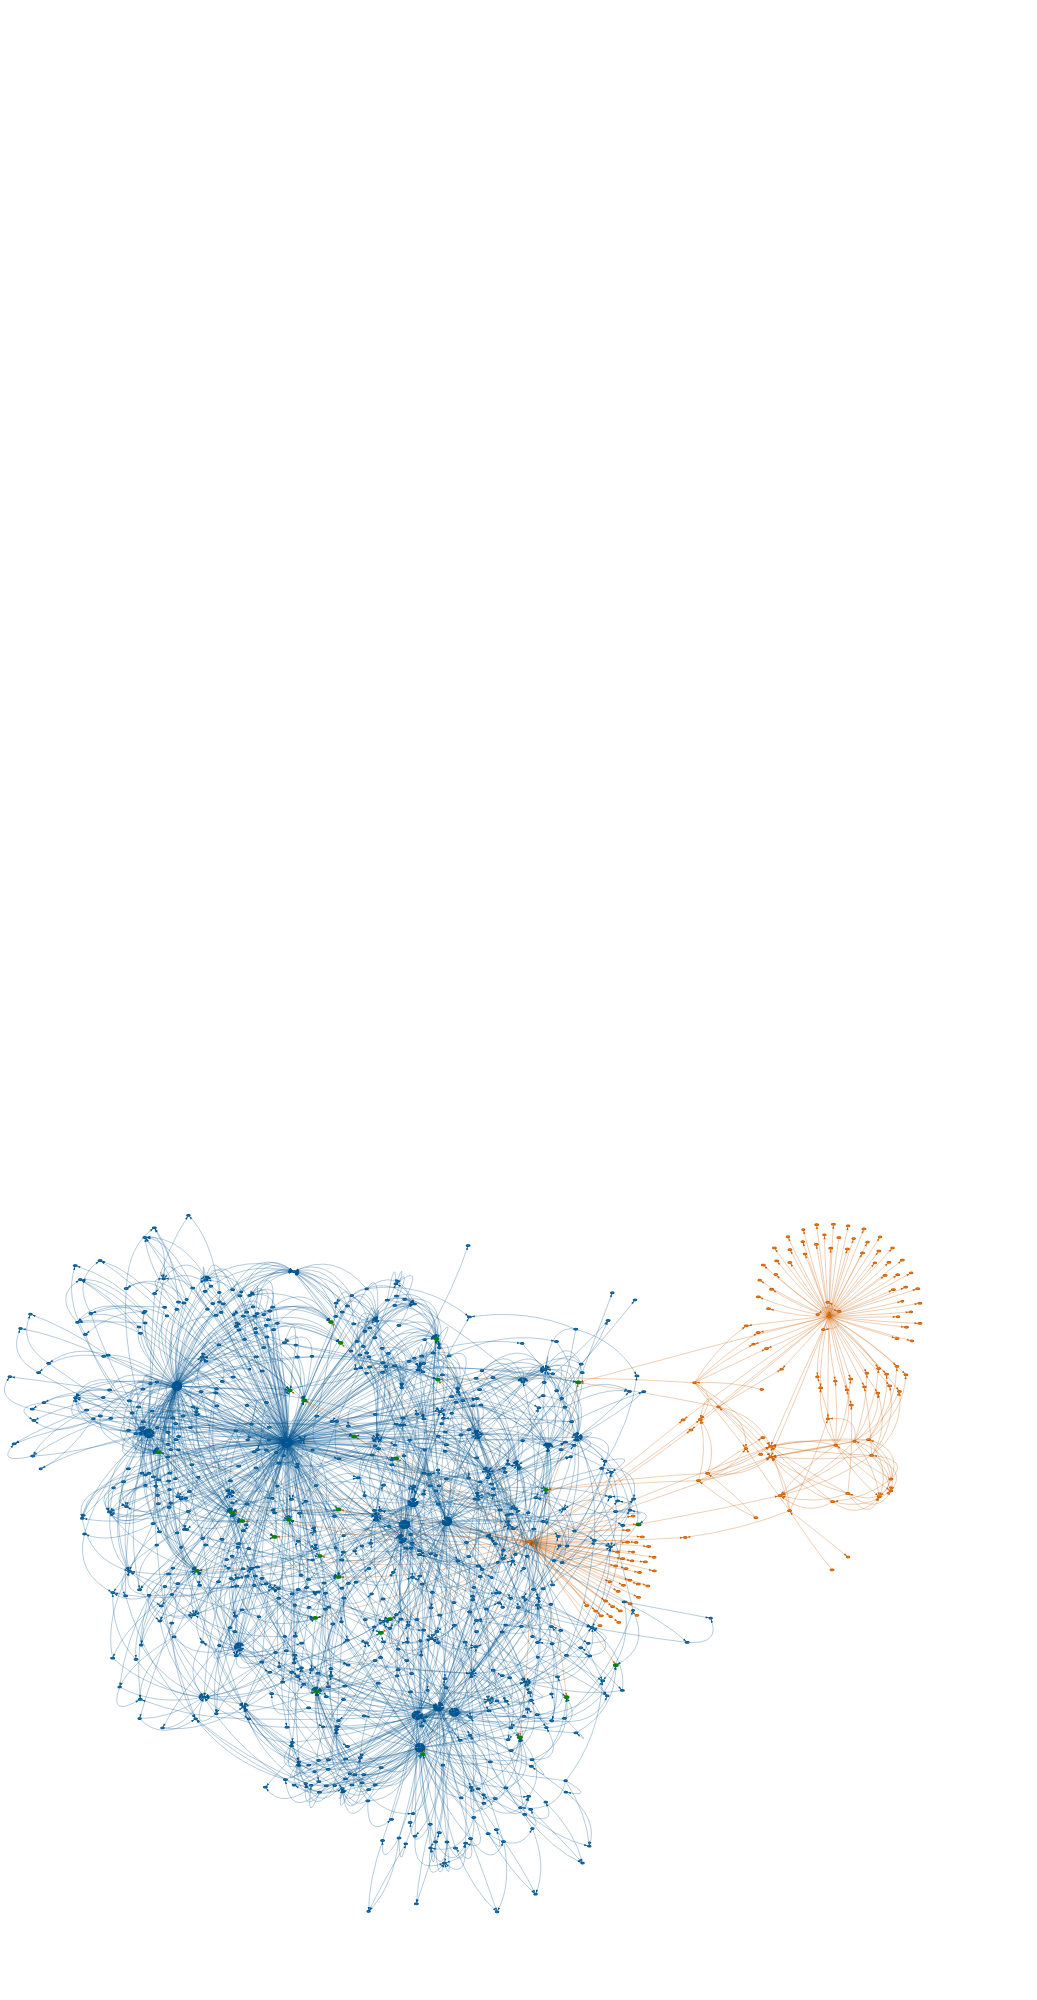
\includegraphics[clip, trim=0cm 3cm 0cm 42cm, width=0.75\textwidth]{figs/snap1_newcolors_horizon.png} %,trim=4.5cm 3cm 2.5cm 2cm,clip]
    \caption{Exemplary KG snapshot for the first timestep. Orange nodes are from GTA, blue nodes are from ACLED, and green nodes appear in both datasets. The majority of triples are from ACLED. Both, ACLED and GTA, contain a small number of hub nodes, linking to a significant amount of other nodes.}
    \label{fig:kg_static}
\end{figure}
\subsection{Challenges and Considerations for tKG Forecasting: Analysis Insights}\label{sec:takeaway}
The insights gained from the analysis help to define requirements for tKG Forecasting for the use case in Section~\ref{sec:intro}. 
Compared to the datasets in Section~\ref{sec:rel_work}, a tKG forecasting model for the given tKG dataset needs to handle a larger number of triples, and a significantly larger number of nodes. Moreover, the model must be capable of distinguishing hub nodes with a very high node degree from nodes with a low node degree, and of differentiating between these. 
Further, the model must be able to account for peak days and incorporate them into its predictions. An additional challenge is the capturing of seasonal information. For this reason, the forecasting model should have the capability to incorporate seasonal variations in its predictions.


\section{Conclusion and Future Work}\label{sec:conclusion}
We have presented a novel approach to understanding global crises and trade patterns. For this, our paper outlines the curation process of a tKG from publicly available dynamic data and includes a comprehensive analysis of this tKG. 
Additionally, we have defined requirements for tKG forecasting models to be used with this dataset.

Leveraging tKG is a promising way to understand the intersection between global crises and trade data over time. 
In the future, we plan to apply tKG forecasting models within the CoyPu project to predict future trade alert events based on the historical global trade and crisis data, taking into account the key takeaways highlighted in Section~\ref{sec:takeaway}. 
Our ultimate goal is to enhance our understanding of crises and trade patterns and to contribute to a more effective decision-making process in response to emerging crises.


\begin{acknowledgments}
The authors acknowledge funding by the Federal Ministry for Economics and Climate Action of Germany in the project CoyPu (project number 01MK21007[A-L]).
\end{acknowledgments}

\bibliography{references}

\end{document}
